\documentclass[letterpaper, 11pt]{article}
\usepackage{helvet}
\usepackage[margin=0.75in]{geometry}
\usepackage{datetime}
\usepackage{natbib}
\usepackage{graphicx}
\usepackage{subfigure}
\usepackage{caption}
\usepackage{amsfonts}
\usepackage{authblk}
\usepackage{enumerate}
\usepackage[colorlinks=true]{hyperref}
\pagestyle{plain}
\pagenumbering{arabic}
\bibliographystyle{plain}

\title{Test Inhibitor Time Course Inference\\Using Gradient Boosted Decision Trees}

\author[1]{Kevin Emmett\thanks{kje2109@columbia.edu}}
\author[2]{Sakellarios Zairis\thanks{siz2102@columbia.edu}}
\affil[1]{Department of Physics, Columbia University}
\affil[2]{Department of Computational Biology \& Bioinformatics, Columbia University}

\setcounter{section}{-1}

\begin{document}

\maketitle

%%%%%%%%%%%%%%%%%%%%%%%%%%%%%%%%%%%%%%%%%%%%%%%%%%%
\section{Summary}

We use a supervised learning technique known as gradient tree boosting to predict forward steps in the time series data, which are represented as pairs of successive time points under a Markov assumption.

%%%%%%%%%%%%%%%%%%%%%%%%%%%%%%%%%%%%%%%%%%%%%%%%%%%
\section{Methods}

\subsection{Relation to Subchallenge 1}

We do not make explicit use of the network edges inferred in subchallenge 1, though the network structure is still latent within our trained gradient boosted trees.

\subsection{Background}

The general gradient boosting tree algorithm is as follows \citep{Hastie2004}:

\begin{enumerate}
\item Initialize $f_{0}(x) = \arg\min_{\gamma}\sum_{i=1}^N L(y_{i}, \gamma)$
\item For $m=1$ to $M$:
  \begin{enumerate}[(a)]
    \item For $i=1,2,\cdots,N$ compute
      \begin{equation}
        r_{im} = -\left[\frac{\partial L(y_{i},f(x_{i}))}{\partial f(x_{i})}\right]_{f=f_{m-1}}
      \end{equation}
    \item Fit a regression tree to the targets $r_{im}$ giving terminal regions $R_{jm}$, $j=1,2,\cdots,J_m$.
    \item For $j=1,2,\cdots,J_{m}$ compute
      \begin{equation}
        \gamma_{jm} = \arg\min_{\gamma}\displaystyle\sum_{x_{i}\in R_{jm}} L(y_{i}, f_{m-1}(x_{i})+\gamma)
      \end{equation}
    \item Update $f_{m}(x) = f_{m-1}(x) + \sum_{j=1}^{J_m} \gamma_{jm} I(x\in R_{jm})$.
  \end{enumerate}
\item Output $\hat{f}(x) = f_{M}(x)$
\end{enumerate}

The salient features of this algorithm are (a) it builds a strong classifier from an ensemble of weaker ones, (b) it re-weights the training data at each iteration to emphasize hitherto incorrectly classified examples, and (c) the final classifier provides not only the $sign$ but also its margin, or distance from zero, as a measure of confidence in the prediction.

\begin{figure}
  \centering
  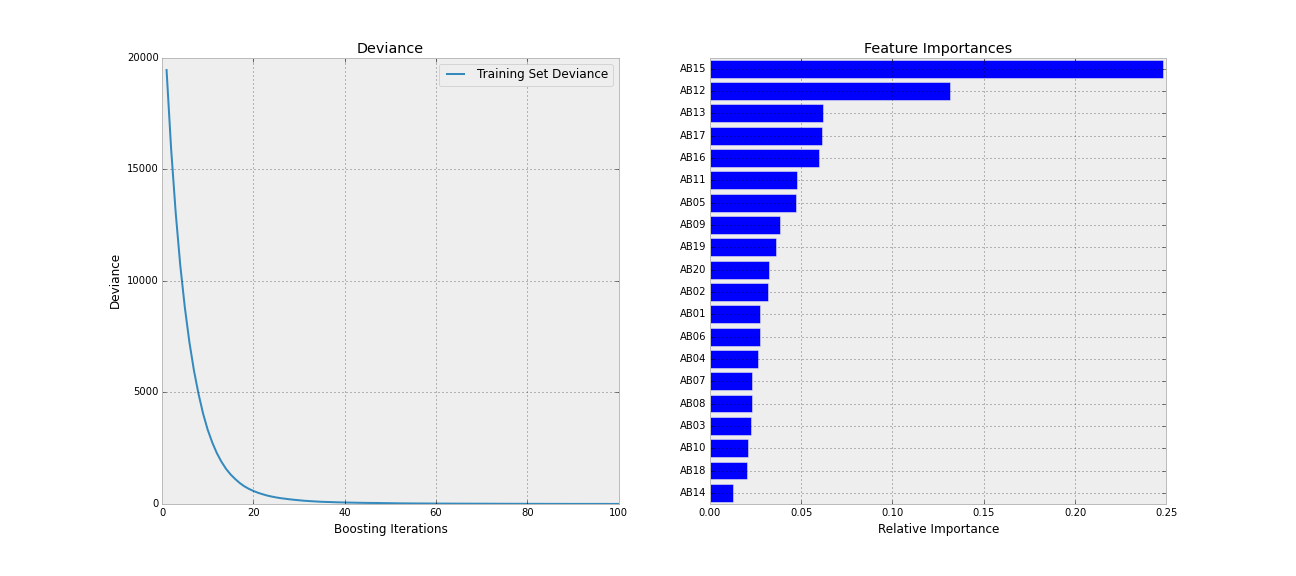
\includegraphics[width=1.0\textwidth]{deviance_feature_importance.png}
  \caption{Training the GBR model for insilico dataset, AB15. Left: Training set deviance for GBR model as function of boosting round. Right: Feature importance rankings.}
\end{figure}
\subsection{Implementation}

Our models were written in python. We used \href{http://pandas.pydata.org/}{pandas} to manipulate the data prior to training, and implemented our models using \href{http://scikit-learn.org/stable/}{scikit-learn}.

\subsection{Parameter Tuning}

Gradient Boosted Decision trees have the following parameters:
\begin{itemize}
  \item \texttt{num\_estimators}: number of rounds of boosting rounds to perform.
  \item \texttt{max\_depth}: maximum depth of the base learners.
  \item \texttt{learning\_rate}: the learning rate shrinks the contribution of each tree by the specified value.
\end{itemize}

We used cross validation to set the best values of the parameters for each trained model.

\subsection{Inhibitor/Stimulus Modeling}

Inhibitors were modeled using a perfect fixed-effects model \citep{Spencer2012}. The stimulus was not explicitly modeled. We dealt with stimulii in two ways: by grouping datasets across stimulii, and by training independent models for each stimulus. We found training separate models for each stimulus performed better.

\subsection{Experimental vs inSilico}

For subchallenge 2, we used the same approach in both 2A and 2B. No prior was user for 2A.

\subsection{Any other approaches considered?}

Our first approach to modeling time series were based on symbolic regression using the genetic algorithm package \href{http://creativemachines.cornell.edu/eureqa}{Eureqa}. While this approach was promising, it was computationally expensive. We also implemented a simple Dynamic Bayesian Network, following \citep{Hill2012}. We found the DBN overfit when used to predict time courses. Before settling on the GBR model, we tried a Lasso regularized linear model, which we found performed slightly worse under cross validation.

\subsection{Computational Resources}

Our algorithms ran on our local machines (Intel Core i7, 8GB RAM), typically taking no more than 5 minutes per run.

%%%%%%%%%%%%%%%%%%%%%%%%%%%%%%%%%%%%%%%%%%%%%%%%%%%
\section{Data Preparation}

For the experimental data, we partitioned the data into independent subsets for each cell line and stimulus combination (\texttt{cell\_line}, \texttt{stim}). We modeled inhibitors using a perfect fixed-effects model \citep{Spencer2012}. We used only the ``Main'' dataset in training our models.

For the insilico data, the dataset was partitioned into independent subsets for each stimulus. Inhibitors were again modeled using a perfect fixed-effects model.

For each dataset, we centered and scaled the columns before training the model. We did not use log-transformed data.

%%%%%%%%%%%%%%%%%%%%%%%%%%%%%%%%%%%%%%%%%%%%%%%%%%%
\section{External Information}

We implemented two literature models of dynamic signaling networks: a 16 node ERK pathway \citep{Xu2010} and a 5 node yeast network \citep{Cantone2009}. We used these as gold standard networks to prototype our model. In these datasets, we had a known network structure which  we used to simulate synthetic time courses.

%%%%%%%%%%%%%%%%%%%%%%%%%%%%%%%%%%%%%%%%%%%%%%%%%%%
\section{Model Validation}

We used k-fold cross validation to test our model performance (k=5, k=10, LOO). We did not model randomness in our cross-validation.

%%%%%%%%%%%%%%%%%%%%%%%%%%%%%%%%%%%%%%%%%%%%%%%%%%%
\section{Leader Board}

We found that our internal cross-validation did map to leaderboard performance. In subchallenge 2A, we participated in all but the first week of the leaderboard. In subchallenge 2B, we participated in all but the last week of the leaderboard. We found the results of the leaderboard useful for gauging relative performance of the teams, but did not find we had enough submissions to creatively iterate on our model.

%%%%%%%%%%%%%%%%%%%%%%%%%%%%%%%%%%%%%%%%%%%%%%%%%%%
\section{Discussion}

We implemented code to use the gradient of the concentration as the output variable, but didn't get a chance to fully test it. We were also interested in using a bootstrap approach where inferred networks from GBR are used to build ODEs for time course prediction. We are pleased nonetheless at our fairly successful application of a powerful method like gradient tree boosting to the domain of network inference where it appears under-utilized.  We anticipate strong performance of this approach as the number of phosphoproteins reported on RPPA chips increases and the danger of overfitting in other methods increases.

%%%%%%%%%%%%%%%%%%%%%%%%%%%%%%%%%%%%%%%%%%%%%%%%%%%
\section{Author Backgrounds and Statements}

Kevin Emmett is a PhD student in physics with a background in discriminative modeling of emerging pathogens. Sakellarios Zairis is an MD/PhD student with a background in applying supervised learning techniques to predicting viral oncogenic potential.  These authors contributed equally to the work, with an average weekly time commitment of 15 hours.

\bibliography{DREAM8}

\end{document}
